\section{\chameleon{} Prototype and RVSI Protocol}

% System Design of \chameleon{}

%%%%%%%%%%%%%%%
\begin{frame}{}
  \begin{center}
    \chameleon{} prototype: \\[10pt]
    A prototype \textbf{partitioned} \textbf{replicated} \\[6pt]
    distributed transactional \textbf{key-value} store
  \end{center}
\end{frame}
%%%%%%%%%%%%%%%

%%%%%%%%%%%%%%%
\begin{frame}{}
  \begin{center}
    Classic \textbf{key-value} data model \\[4pt]
      Key: (row key, column key)
  \end{center}
\end{frame}
%%%%%%%%%%%%%%%

%%%%%%%%%%%%%%%
\begin{frame}{}
  % \fignocaption{width = 0.70\textwidth}{figs/chameleon-arch.pdf}
  \begin{center}
    \resizebox{0.70\textwidth}{!}{%        File: chameleon-arch.tex
%     Created: Mon Jan 04 08:00 PM 2016 C
% Last Change: Mon Jan 04 08:00 PM 2016 C
% 	    Used in Beamer

\begin{tikzpicture}[connection/.style = {>=Stealth, <->, brown, dashed, line width = 3pt}]
  % background: china map
  \node (china-map) [opacity = 0.20] {
\includegraphics[scale = 0.40]{figs/china-outline-blue.png}};

  % partition-left, partition-right, partition-below
  \uncover<2->{
    \node (partition-left) [] at (-6.5, 1) {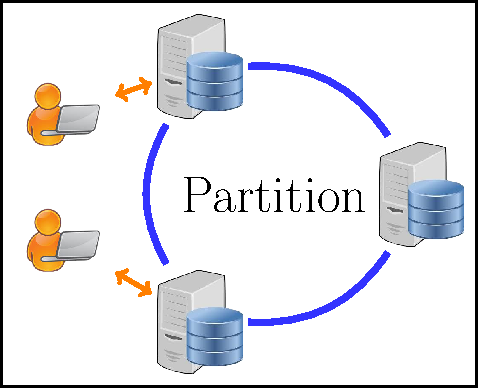
\includegraphics[scale = 0.80]{figs/partition.pdf}}; 
  }
  \uncover<3->{
    \node (partition-right) [] at (6, 3.5) {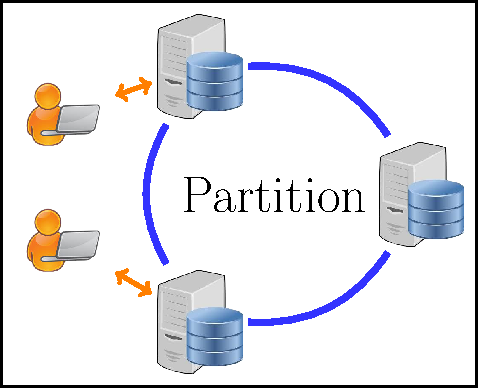
\includegraphics[scale = 0.80]{figs/partition.pdf}}; 
    \node (partition-below) [] at (1.5, -5) {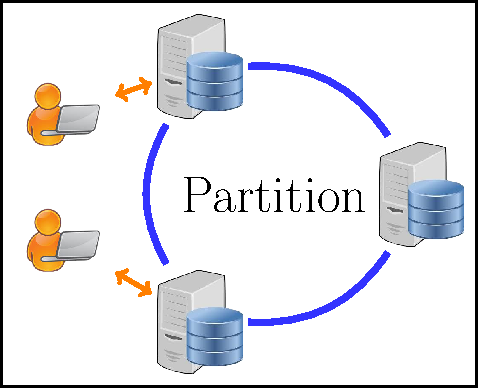
\includegraphics[scale = 0.80]{figs/partition.pdf}}; 

    % connections among partitions
    \draw [connection] (partition-left) to (partition-right); 
    \draw [connection] (partition-right) to (partition-below);
    \draw [connection] (partition-below) to (partition-left);

    % replication 
    \node (replication) [font = \Huge, align = center] at (0.5, 0.0) {\textbf{Wide-area}\\[3pt]\textbf{Replication}};
  }

  \uncover<4->{
    % master-slave for one partition
    \begin{scope}[circled/.style = {draw, circle, dash pattern = on 10pt off 5pt, cyan, line width = 2pt, outer sep = 5pt, minimum size = 2.0cm}, 
      conn/.style = {dash pattern = on 15pt off 8pt, cyan, line width = 2pt}]
    \node (ms-left) [circled] at (-4., 1) {};
    \node (ms-right) [circled] at (5.5, 1.7) {};
    \node (ms-below) [circled] at (4., -5.0) {};

    \node (master-slave) [below right = 1.5cm and -1.5cm of partition-right] {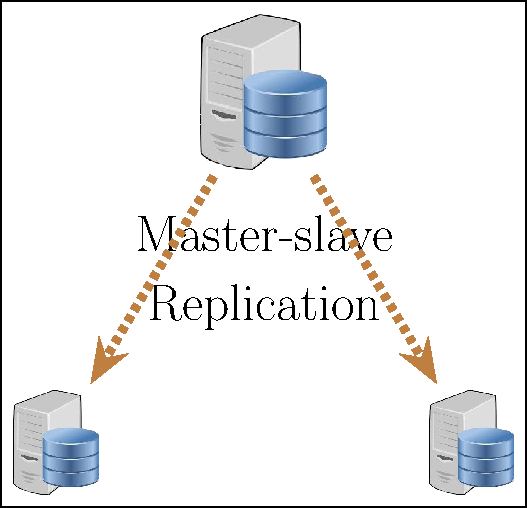
\includegraphics[scale = 0.80]{figs/master-slave.pdf}};
    \draw [conn] (ms-left) to (master-slave);
    \draw [conn] (ms-right) to (master-slave);
    \draw [conn] (ms-below) to (master-slave);
    \end{scope}
  }
\end{tikzpicture}
}
  \end{center}

  \begin{center}
    \only<2>{Keys are \textbf{partitioned} within a single datacenter.}
    \only<3-4>{Each key is \textbf{replicated} across datacenters} \only<4>{in a \textbf{master-slave} manner.}
    \only<5>{Transactions are first executed and committed on the \textbf{masters},\\
      and are then asynchronously propagated to \textbf{slaves}.}
  \end{center}
\end{frame}
%%%%%%%%%%%%%%%

%%%%%%%%%%%%%%%
\begin{frame}{}
  \only<1-3, 5->{\fignocaption{width = 0.50\textwidth}{figs/chameleon-framework.pdf}}

  \begin{center}
    \only<2>{\blue{1.} Partitioned replicated transactional key-value store}
    \only<3>{\blue{2.} Client library}
    \only<5>{\blue{3.} \rvsi{} protocol: \rvsims{} + \rvsimp{}}
  \end{center}

  \only<4>{
    Code snippet for writing \rvsi{} transactions: \\[8pt]
    \begin{lstlisting}[
  language = Java,
  basicstyle = \ttfamily\footnotesize,
  showstringspaces = false,
  keywordstyle = \color{blue}\bfseries,
  commentstyle = \color{teal},
  stringstyle = \bfseries,
  upquote = true,
  frame = box,
  breaklines = true,
  linewidth = 0.85\textwidth
]
  // Initialize keys (ck, ck1, and ck2) here
  ITx tx = new RVSITx(/** context **/);

  tx.begin();

  // Read and write
  ITsCell tsCell = tx.read(ck);
  ITsCell tsCell1 = tx.read(ck1);
  tx.write(ck1, new Cell("R1C1"));
  ITsCell tsCell2 = tx.read(ck2);

  // Specify RVSI specs. (e.g., SVSpec)
  RVSISpec sv = new SVSpec();
  sv.addSpec({ck, ck1, ck2}, 2);
  tx.collectRVSISpec(sv);

  boolean committed = tx.end();
\end{lstlisting}

  }
\end{frame}
%%%%%%%%%%%%%%%


% the RVSI-MS protocol
%%%%%%%%%%%%%%%
\begin{frame}{}
  \centerline{\rvsims{}: RVSI protocol for Master-Slave replication}

  \vspace{-0.80cm}
  \begin{center}
    \resizebox{0.50\textwidth}{!}{\begin{tikzpicture}[
  msg/.style = {>=Stealth, <->, very thick}]
  \node (ms) [] {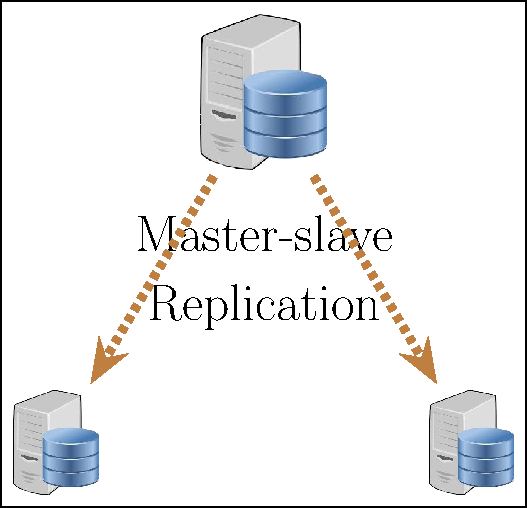
\includegraphics[scale = 0.40]{figs/master-slave.pdf}};
  \node (client) [above = 2.0cm of ms] {
\includegraphics[scale = 0.25]{figs/client-pc-logo.png}};

  \uncover<2->{
    % begin
    \draw [msg] (client) to node () [below = 5pt, midway, sloped] {\textsc{Begin}} 
    node () [above = 5pt, midway, sloped] {$T$.sts} (ms);
  }

  \uncover<3->{
    % read
    \draw [msg] (client) to [bend right = 40] node () [above = 5pt, midway, sloped] {\textsc{Read}} 
    ($(ms.south west) + (0,20pt)$);
  }

  \uncover<4->{
    % write
    \draw [msg] (client) to [out = -30, in = 30, looseness = 5] node () [] {\textsc{Write}} (client);
  }

  \uncover<5->{
    % commit
    \draw [msg] (client) to [bend left = 60] node () [below = 5pt, midway, sloped] {\textsc{Commit}} 
    node () [above = 5pt, midway, sloped] {$T$.cts} ($(ms.north) + (25pt, 0)$);
  }

  \uncover<6->{
    % vc
    \node () [below right = 0.10cm and 0.20cm of client.south, red] {$\textsc{ADD-VC}$};
    \node () [below right = 0.50cm and 0.20cm of ms.north, red] {\textsc{CHECK-VC}};
  }
\end{tikzpicture}}
  \end{center}

%   \vspace{1.0cm}
%   In terms of \emph{event} generation and handling:
%   \begin{description}
%     \item[Clients:] \ebegin, \eread, \ewrite, \eend%
%     \item[Master:] \estart, \ecommit, \esend%
%     \item[Slaves:] \ereceive%
%   \end{description}
\end{frame}
%%%%%%%%%%%%%%%

%%%%%%%%%%%%%%%
\begin{frame}{}
  Calculating version constraints for \rvsi{}: 

  \[
    \mathcal{O}_{x}(t) = \text{\# of versions of } x \text{ before time } t % \max \set{x.\attr{ord} \mid x.\attr{ts} \le t}
  \]

  \[
    \blue{r_i(x_j) \in T_i}
  \]
  \vspace{-0.40cm}
  \begin{description}
    \item[$\konebv$:]
      \[
	\mathcal{O}_{x}(T_i.\textsl{sts}) - \mathcal{O}_{x}(T_j.\textsl{cts}) < k_1
      \]
    \item[$\ktwofv$:]
      \[
	\mathcal{O}_{x}(T_j.\textsl{cts}) - \mathcal{O}_{x}(T_i.\textsl{sts}) \le k_2
      \]
    \pause
    \item[$\kthreesv$:]
      \[
	\blue{r_i(x_j), r_i(y_l) \in T_i}
      \]
      \vspace{-0.40cm}
      \[
	\mathcal{O}_{\red{x}}(T_l.\textsl{cts}) - \mathcal{O}_{\red{x}}(T_j.\textsl{cts}) \le k_3
      \]
  \end{description}
\end{frame}
%%%%%%%%%%%%%%%

% the RVSI-MP protocol
%%%%%%%%%%%%%%%
\begin{frame}{}
  \begin{center}
    \rvsimp{}: \rvsi{} protocol for Multiple Partitions\\[10pt]
    Distributed transactions spanning multiple masters \\
    need to be committed atomically.

    \pause
    \vspace{0.40cm}
    Using the two-phase commit (2PC) protocol \citeinbeamer{Bernstein}{Book}{87}.

    \pause
    \vspace{1.00cm}
    We have two issues to address.
  \end{center}
\end{frame}
%%%%%%%%%%%%%%%

%%%%%%%%%%%%%%%
\begin{frame}{}
  Assumes a timestamp oracle \citeinbeamer{Peng}{OSDI}{10}:
  \begin{description}[Coordinator:]
    \item[Client:] asks for the start-timestamp in \textsc{Begin}
    \item[Coordinator:] asks for the commit-timestamp in \textsc{Commit}
  \end{description}
\end{frame}
%%%%%%%%%%%%%%%

%%%%%%%%%%%%%%%
\begin{frame}{}
  Split the \rvsi{} version constraints according to partitions:

  \[
    \blue{r_i(x_j) \in T_i}
  \]
  \vspace{-0.40cm}
  \begin{description}
    \item[$\konebv$:]
      \[
	\mathcal{O}_{\red{x}}(T_i.\textsl{sts}) - \mathcal{O}_{\red{x}}(T_j.\textsl{cts}) < k_1
      \]
    \item[$\ktwofv$:]
      \[
	\mathcal{O}_{\red{x}}(T_j.\textsl{cts}) - \mathcal{O}_{\red{x}}(T_i.\textsl{sts}) \le k_2
      \]
    \item[$\kthreesv$:]
      \[
	\blue{r_i(x_j), r_i(y_l) \in T_i}
      \]
      \vspace{-0.40cm}
      \[
	\mathcal{O}_{\red{x}}(T_l.\textsl{cts}) - \mathcal{O}_{\red{x}}(T_j.\textsl{cts}) \le k_3
      \]
  \end{description}

  \vspace{0.6cm}
  \centerline{All version constraints involve only one data item.}
\end{frame}
%%%%%%%%%%%%%%%
